\documentclass[aspectratio=169,11pt]{beamer}

\usepackage[utf8]{inputenc}
\usepackage[T1]{fontenc}
\usepackage[french]{babel}
\usepackage{graphicx}
\usepackage{listings}
\usepackage{booktabs}
\usepackage{tikz}
\usetikzlibrary{shapes.geometric, arrows, positioning}

% Theme Madrid + couleurs rapport
\usetheme{Madrid}
\usecolortheme{seahorse}
\definecolor{burgundy}{HTML}{8e5e2d}
\definecolor{gold}{HTML}{4c1207}
\setbeamercolor{structure}{fg=burgundy}
\setbeamercolor{title}{fg=white,bg=burgundy}
\setbeamercolor{frametitle}{fg=white,bg=burgundy}
\setbeamercolor{block title}{fg=white,bg=burgundy}
\setbeamercolor{block body}{bg=burgundy!5}
\setbeamercolor{block title example}{fg=white,bg=gold}
\setbeamercolor{block body example}{bg=gold!5}
\setbeamercolor{itemize item}{fg=burgundy}

% Code
\lstset{
    language=C++,
    basicstyle=\ttfamily\scriptsize,
    keywordstyle=\color{burgundy}\bfseries,
    commentstyle=\color{green!50!black}\itshape,
    frame=single,
    rulecolor=\color{burgundy!30},
    backgroundcolor=\color{burgundy!3},
    breaklines=true,
    showstringspaces=false,
    morekeywords={__global__,__device__,__host__,__shared__,__constant__,__align__,
                  parallel,task,single,for,critical,atomic,
                  thread_local,KOKKOS_INLINE_FUNCTION,Kokkos,View,parallel_for,
                  uint64_t,u64,u8},
}

\setbeamertemplate{navigation symbols}{}

% Background transparent sur toutes les slides
\usebackgroundtemplate{%
  \begin{tikzpicture}[remember picture,overlay]
    \node[opacity=0.06, anchor=south] at ([shift={(0,-1cm)}]current page.south) {%
      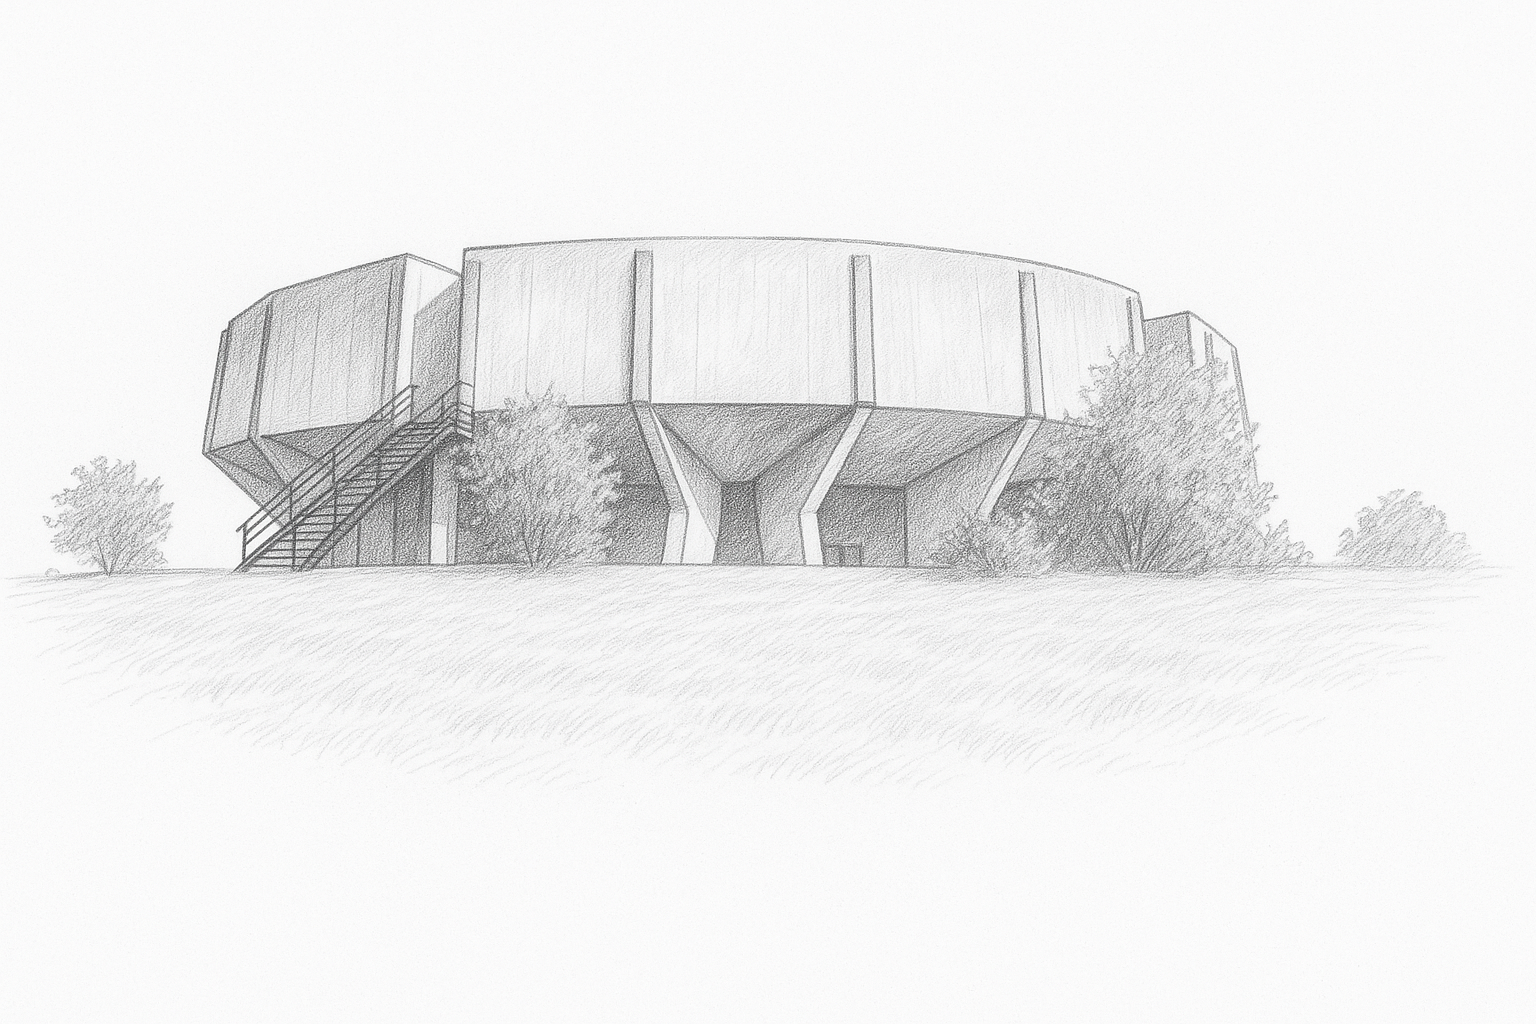
\includegraphics[width=\paperwidth,keepaspectratio]{assets/back.png}%
    };
  \end{tikzpicture}%
}

% Footer avec nom + CHPS + page
\setbeamertemplate{footline}{%
  \leavevmode%
  \hbox{%
    \begin{beamercolorbox}[wd=.4\paperwidth,ht=2.5ex,dp=1ex,leftskip=1em]{author in head/foot}%
      \usebeamerfont{author in head/foot}\insertshortauthor{} -- CHPS0801%
    \end{beamercolorbox}%
    \begin{beamercolorbox}[wd=.6\paperwidth,ht=2.5ex,dp=1ex,rightskip=1em]{date in head/foot}%
      \hfill\usebeamerfont{date in head/foot}\insertframenumber/\inserttotalframenumber%
    \end{beamercolorbox}%
  }%
}

\title{Wave Function Collapse}
\subtitle{Modèle overlapping : Séquentiel, OpenMP \texttt{task}, Kokkos CPU+GPU}
\author{Despoullains, Marano}
\institute{Université de Reims Champagne-Ardenne\\M1 CHPS -- CHPS0801 Modèles de programmation parallèle}
\date{2025--2026}

\begin{document}

% ============================================================
\begin{frame}[plain]
\begin{tikzpicture}[remember picture,overlay]
% Logos en haut
\node[anchor=north west] at ([shift={(0.3cm,-0.15cm)}]current page.north west) {%
  
\includegraphics[height=0.75cm]{assets/logo-urca.png}%
};
% Ligne de séparation en bas
\draw[burgundy, line width=0.5pt]
  ([shift={(0.5cm,1.2cm)}]current page.south west) --
  ([shift={(-0.5cm,1.2cm)}]current page.south east);
% Info en bas
\node[anchor=south west] at ([shift={(0.5cm,0.4cm)}]current page.south west) {%
  {\color{burgundy}\scriptsize CHPS0801 : Modèles de programmation parallèle}%
};
\node[anchor=south east] at ([shift={(-0.5cm,0.4cm)}]current page.south east) {%
  {\color{burgundy}\scriptsize 2025-2026}%
};
\end{tikzpicture}

\vspace{1cm}

{\color{burgundy}\fontsize{20}{24}\selectfont\bfseries Wave Function Collapse}\\[0.1cm]
{\color{burgundy}\rule{0.6\textwidth}{1pt}}\\[0.2cm]
{\color{gold}\normalsize\bfseries Modèle overlapping : Séquentiel, OpenMP \texttt{task}, Kokkos CPU + GPU}\\[0.5cm]

{\itshape\color{black}\large Romain Despoullains, Nicolas Marano}
\hfill
\raisebox{-1.5cm}{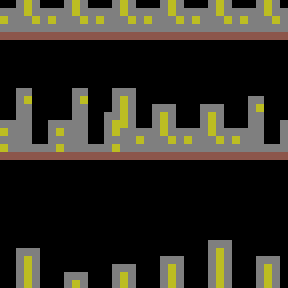
\includegraphics[width=5cm]{results/figures/results/gallery/skyline_seed42.png}}

\vfill
\end{frame}

% ============================================================
\begin{frame}{Sommaire}
\setbeamercolor{section in toc}{fg=black}
\setbeamercolor{subsection in toc}{fg=burgundy!80!black}
\setbeamertemplate{section in toc}[sections numbered]
\begin{columns}[T]
\begin{column}{0.45\textwidth}
\tableofcontents[sections={1-3}]
\end{column}
\begin{column}{0.02\textwidth}
\centering
\vspace{-0.3cm}
{\color{burgundy}\rule{1.5pt}{0.55\textheight}}
\end{column}
\begin{column}{0.45\textwidth}
\tableofcontents[sections={4-6}]
\end{column}
\end{columns}
\end{frame}

% ============================================================
\section{Le problème WFC}

\begin{frame}{Le problème en une figure}
\begin{columns}[c]
\begin{column}{0.55\textwidth}
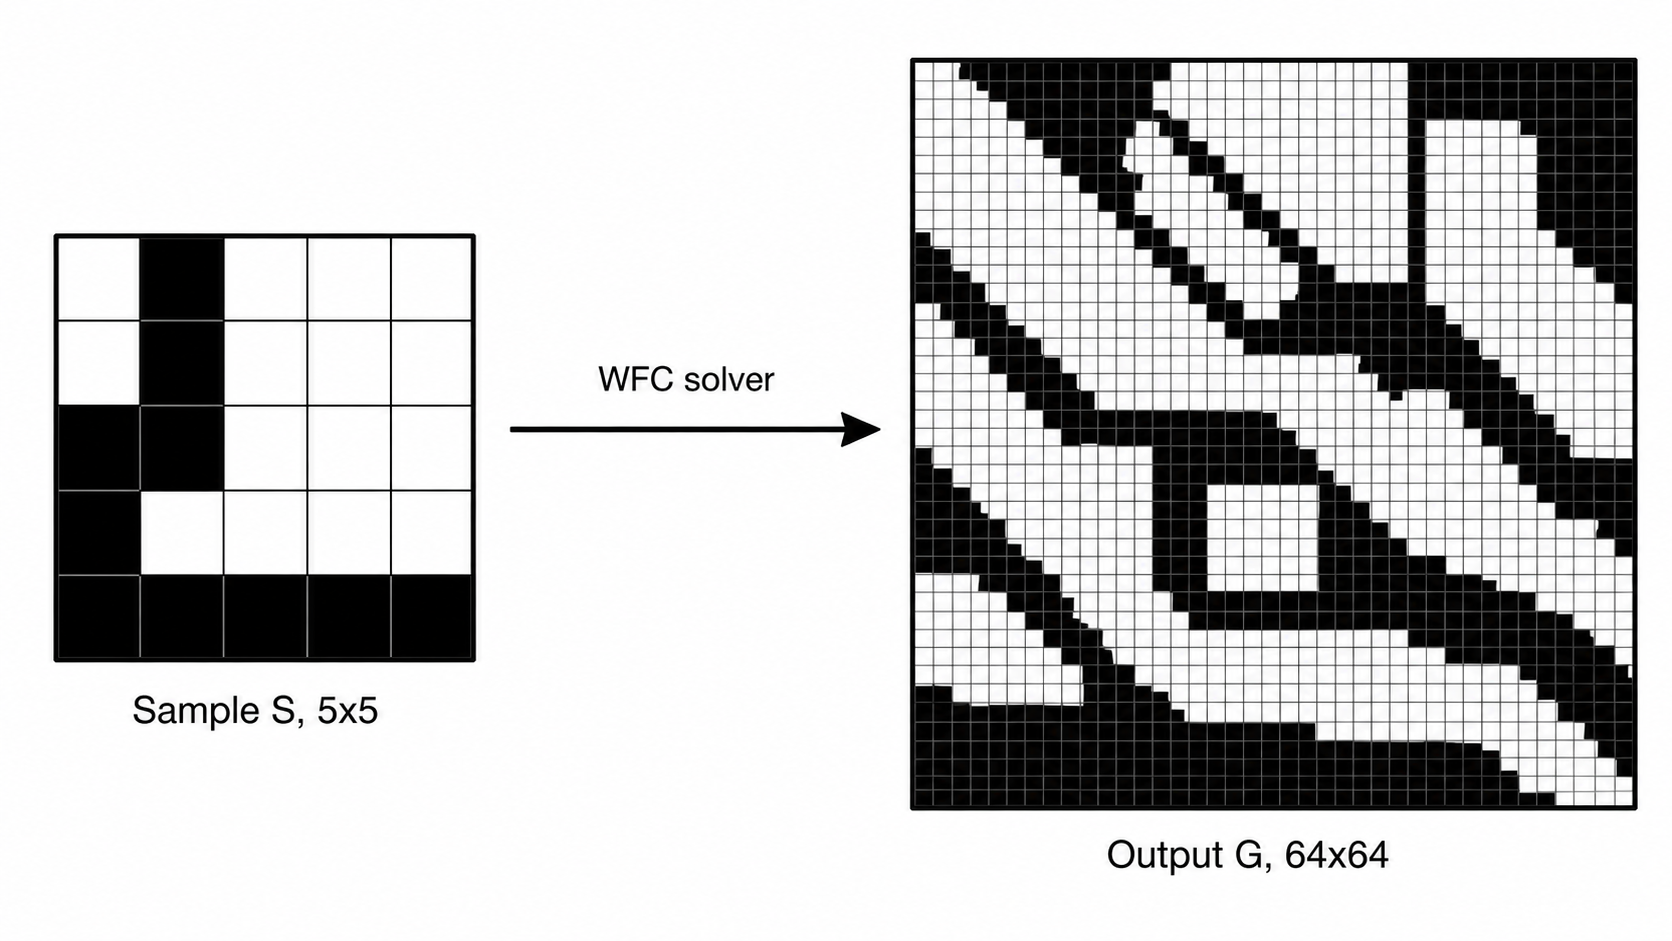
\includegraphics[width=\textwidth]{results/figures/schemas/sample_to_output.png}
\end{column}
\begin{column}{0.42\textwidth}
\textbf{Wave Function Collapse} (Gumin, 2016)
\begin{itemize}
    \item Échantillon $S$ de taille modeste
    \item Paramètre $N$ (taille de tuile)
    \item Sortie $G$ taille libre
    \item Tout sous-bloc $N \times N$ de $G$ apparaît dans $S$
\end{itemize}

\vspace{0.2cm}
\textbf{Modèle overlapping}
\begin{itemize}
    \item Contraintes par recouvrement
    \item $(2N-1)^2$ offsets pertinents
\end{itemize}
\end{column}
\end{columns}
\end{frame}

% ============================================================
\begin{frame}{Compatibilité par overlap}
\begin{columns}[T]
\begin{column}{0.55\textwidth}
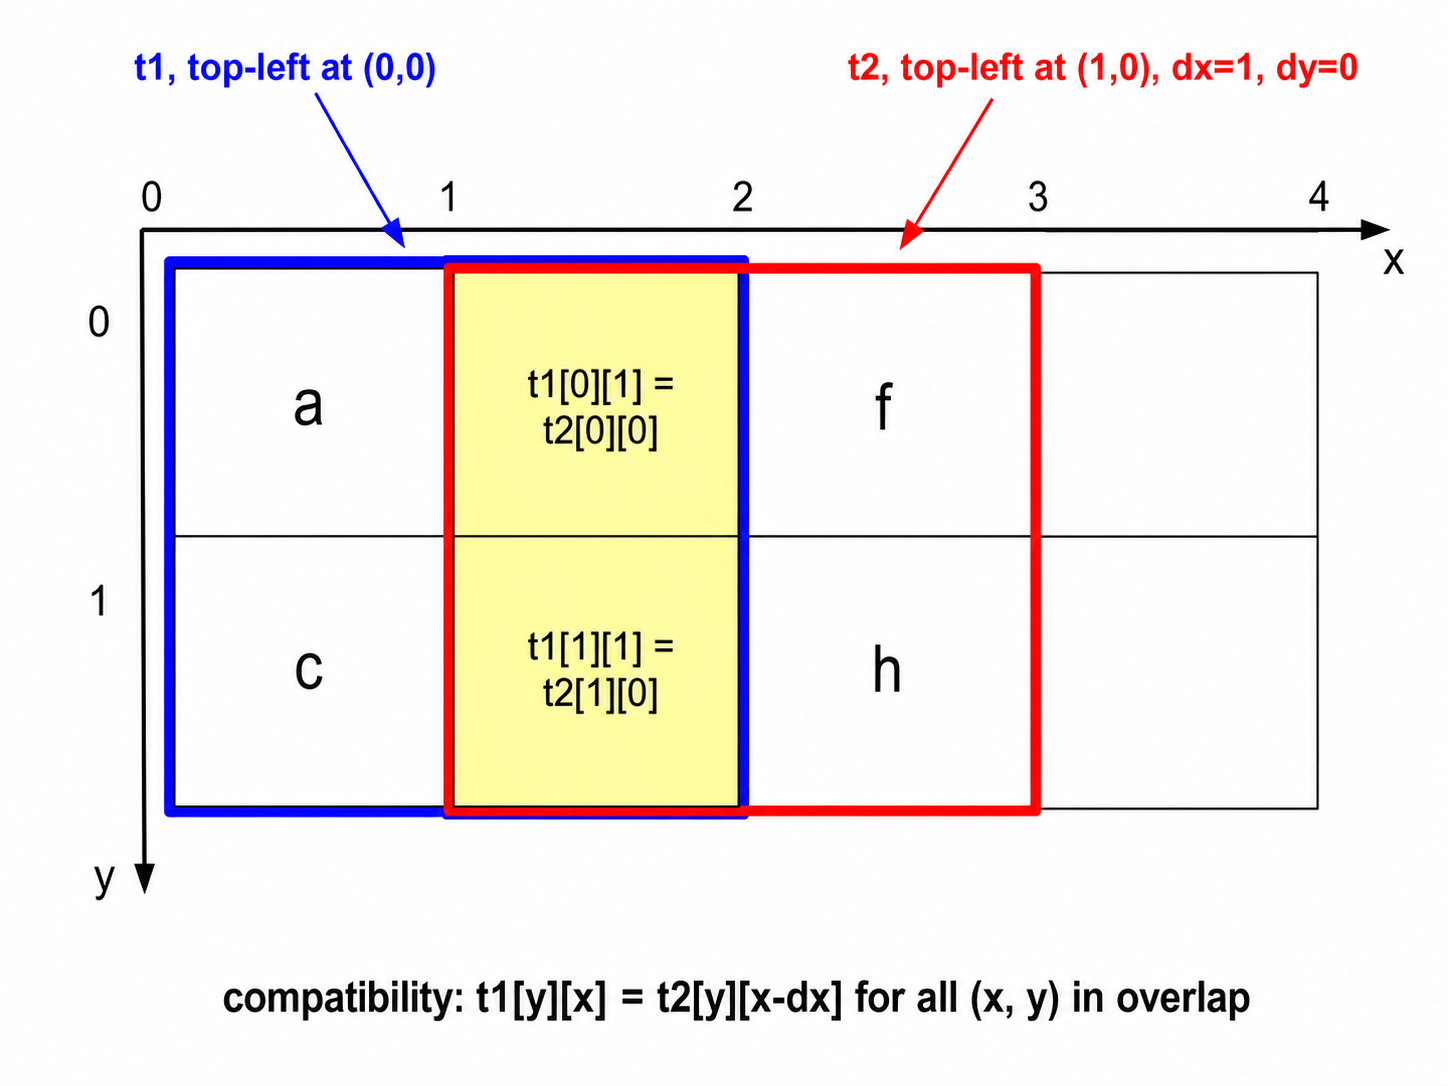
\includegraphics[width=\textwidth]{results/figures/schemas/overlap_compatibility.png}
\end{column}
\begin{column}{0.42\textwidth}
\textbf{Compatibilité} de $t_2$ à offset $(dx, dy)$ de $t_1$ :
\[ t_1[y+dy][x+dx] = t_2[y][x] \]
sur la zone de recouvrement (en jaune).

\vspace{0.2cm}
\textbf{Symétrie des règles :}
\[ t_2 \in \text{allow}(t_1, d) \iff t_1 \in \text{allow}(t_2, -d) \]

\vspace{0.2cm}
\textbf{Stockage :} bitset packé sur \texttt{uint64\_t}, indexé par tuile.
\end{column}
\end{columns}
\end{frame}

% ============================================================
\begin{frame}{Algorithme séquentiel}
\begin{columns}[T]
\begin{column}{0.55\textwidth}
\textbf{Six étapes :}
\begin{enumerate}
    \item Extraction toroïdale des tuiles
    \item Pré-calcul des règles d'adjacence
    \item Init de la wave (toutes tuiles candidates)
    \item Sélection min-entropie + collapse
    \item Propagation BFS niveau-synchrone
    \item Goto 4 jusqu'à convergence
\end{enumerate}

\vspace{0.2cm}
\textbf{Entropie de Shannon pondérée}
\[ H(c) = \log\!\sum_t f_t - \frac{\sum_t f_t \log f_t}{\sum_t f_t} \]

\textbf{Jitter SplitMix64 stateless} (déterminisme à travers backends).
\end{column}
\begin{column}{0.42\textwidth}
\begin{block}{Stratégies de récupération}
\begin{itemize}
    \item Restart-on-contradiction (défaut)
    \item Backtracking + delta snapshot (\texttt{--backtrack})
    \item Parallel attempts (\texttt{--parallel-attempts K})
\end{itemize}
\end{block}
\end{column}
\end{columns}
\end{frame}

% ============================================================
\section{Architecture du code}

\begin{frame}{Architecture : trois libs CMake}
\begin{center}
\begin{tikzpicture}[
    every node/.style={font=\ttfamily\small},
    lib/.style={draw, rounded corners=2pt, fill=burgundy!15, minimum height=0.7cm, inner sep=4pt},
    backend/.style={draw, rounded corners=2pt, fill=gold!15, minimum height=0.7cm, inner sep=4pt},
    arrow/.style={->, >=stealth, burgundy, thick},
    scale=0.9, transform shape,
]
\node[lib] (core) at (0,0) {wfc\_core};
\node[backend] (omp) at (-3.5,-1.8) {wfc\_omp\_lib};
\node[backend] (kokkos) at (3.5,-1.8) {wfc\_kokkos\_lib};
\node[draw, fill=burgundy!5, rounded corners=2pt, font=\ttfamily\scriptsize, minimum height=0.5cm, inner sep=2pt] (s1) at (-6,-3.2) {wfc\_serial};
\node[draw, fill=burgundy!5, rounded corners=2pt, font=\ttfamily\scriptsize, minimum height=0.5cm, inner sep=2pt] (s2) at (-3.5,-3.2) {wfc\_omp};
\node[draw, fill=burgundy!5, rounded corners=2pt, font=\ttfamily\scriptsize, minimum height=0.5cm, inner sep=2pt] (s3) at (3.5,-3.2) {wfc\_kokkos};
\node[draw, fill=burgundy!5, rounded corners=2pt, font=\ttfamily\scriptsize, minimum height=0.5cm, inner sep=2pt] (s4) at (6,-3.2) {wfc\_dungeon};
\draw[arrow] (core) -- (omp);
\draw[arrow] (core) -- (kokkos);
\draw[arrow] (core.south) -- (s1.north);
\draw[arrow] (omp) -- (s2);
\draw[arrow] (kokkos) -- (s3);
\draw[arrow] (core.south) -- (s4.north);
\end{tikzpicture}
\end{center}

\vspace{0.2cm}
\begin{itemize}
    \item \texttt{wfc\_core} : Grid, TileSet, OverlapRules, Wave, Bitset, SolverBase, SolverSerial.
    \item Backends opt-in : \texttt{wfc\_serial} ne lie pas OMP, \texttt{wfc\_omp} ne lie pas Kokkos.
    \item Pattern \textbf{Template Method} : SolverBase tient le retry/stats/dispatch, chaque backend fournit \texttt{pick\_cell()} et \texttt{propagate()}.
\end{itemize}
\end{frame}

% ============================================================
\begin{frame}{Wave : layout flat NUMA-friendly}
\begin{columns}[T]
\begin{column}{0.55\textwidth}
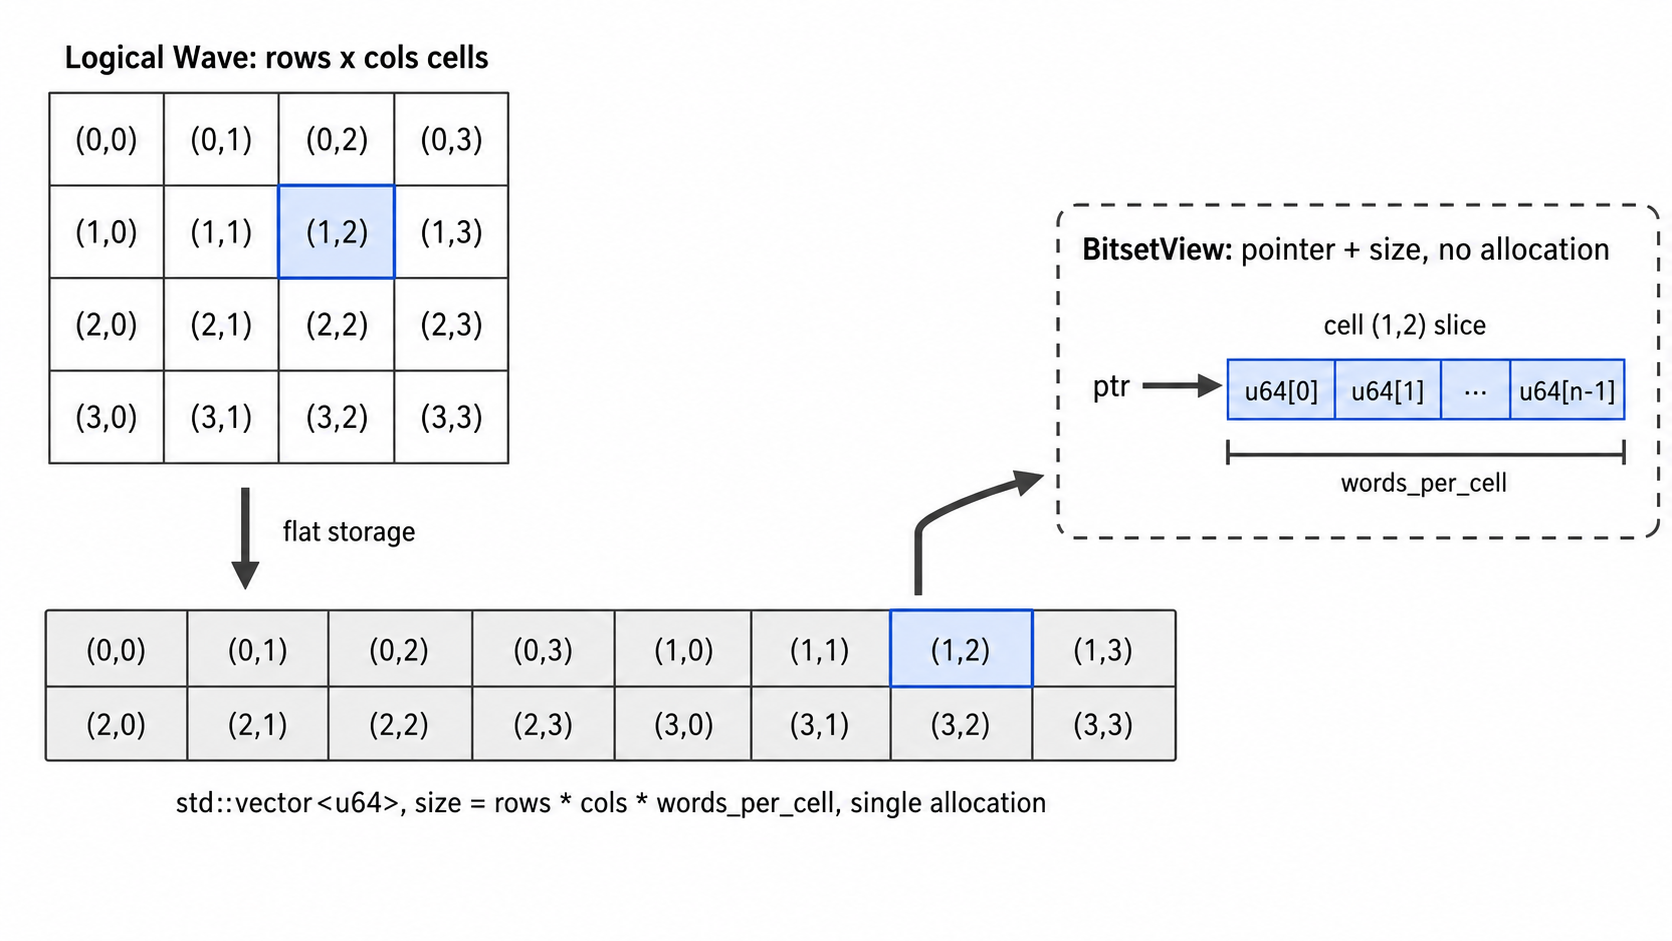
\includegraphics[width=\textwidth]{results/figures/schemas/wave_memory_layout.png}
\end{column}
\begin{column}{0.42\textwidth}
\textbf{Un seul \texttt{vector<u64>} contigu}
\begin{itemize}
\footnotesize
    \item 1 alloc pour toute la wave
    \item \texttt{at(r,c)} renvoie \texttt{BitsetView} (pointeur + taille, sans alloc)
    \item Cache-friendly + NUMA-friendly
\end{itemize}

\vspace{0.2cm}
\textbf{First-touch parallèle}
\begin{itemize}
\footnotesize
    \item \texttt{\#pragma omp parallel for} sur l'init
    \item \texttt{OMP\_PROC\_BIND=close}
    \item Pages mappées aux nœuds NUMA des consommateurs
\end{itemize}
\end{column}
\end{columns}
\end{frame}

% ============================================================
\section{Profilage et OpenMP}

\begin{frame}{Profilage série : où paralléliser ?}
\begin{columns}[T]
\begin{column}{0.45\textwidth}
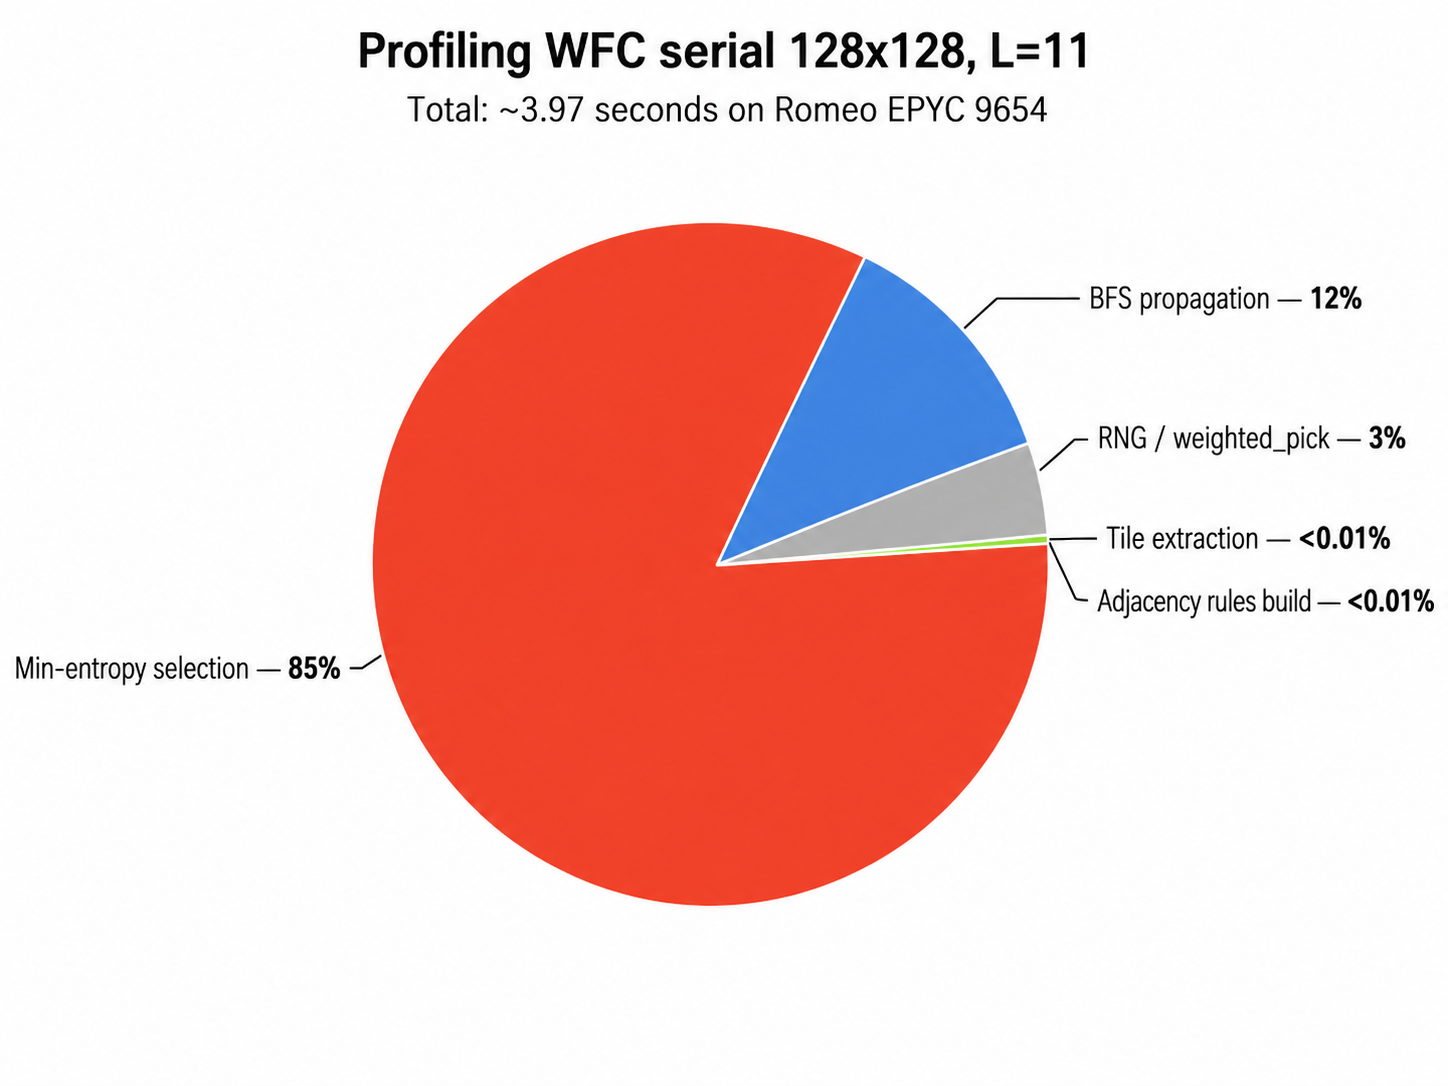
\includegraphics[width=\textwidth]{results/figures/schemas/profile_breakdown.png}
\end{column}
\begin{column}{0.52\textwidth}
\begin{block}{Décomposition du temps -- 128$\times$128, $L=11$}
\centering
\footnotesize
\begin{tabular}{lr}
\toprule
\textbf{Étape} & \textbf{\%} \\
\midrule
\textbf{Sélection min-entropie} & \textbf{$\sim 85\%$} \\
Propagation BFS & $\sim 12\%$ \\
RNG + tirage pondéré & $\sim 3\%$ \\
Extraction tuiles & $< 0.01\%$ \\
\bottomrule
\end{tabular}
\end{block}

\vspace{0.2cm}
\textbf{Conséquence}
\begin{itemize}
    \item L'effort principal porte sur la \emph{sélection}, pas la propagation.
    \item Notre première intuition (\og la propagation domine \fg) était fausse.
\end{itemize}
\end{column}
\end{columns}
\end{frame}

% ============================================================
\begin{frame}[fragile]{OMP : sélection min-entropie chunkée}
{\scriptsize\textbf{1 chunk = 1 task = 1 thread.} Réduction en ordre de chunk fixe = déterminisme bit-à-bit. Short-circuit en série sous 50k ops.}
\begin{lstlisting}
#pragma omp parallel shared(wave, freq, partials)
{
    #pragma omp single
    for (int k = 0; k < n_chunks; ++k) {
        #pragma omp task firstprivate(k)
        {
            MinEntropyResult best;
            for (int c = k*chunk; c < (k+1)*chunk; ++c) {
                if (wave.at(c).count() <= 1) continue;
                double key = weighted_entropy(wave.at(c), freq)
                           + cell_jitter(c, seed);
                if (key < best.value) { best.value = key; best.cell = c; }
            }
            partials[k] = best;
        }
    }
}
// Reduction in fixed chunk order : deterministic.
for (auto& p : partials) if (p.value < global.value) global = p;
\end{lstlisting}
\end{frame}

% ============================================================
\begin{frame}[fragile]{OMP : une seule région \texttt{parallel}}
\begin{block}{Le problème}
Région \texttt{parallel} par niveau BFS = $\sim 50\,\mu s$ fork/join $\times$ 8000 niveaux $= 400\,$ms d'overhead pur. Plus que le travail utile total.
\end{block}

\begin{lstlisting}
#pragma omp parallel shared(frontier, next, wave, rules, ...)
{
    while (!finished) {
        const int chunk     = std::max(1, frontier_size / (4 * max_threads));
        const bool use_tasks = frontier_size >= kSerialFallback;

        #pragma omp single
        {
            if (!use_tasks) serial_pass(frontier, ...);  // frontier-threshold
            else for (int s = 0; s < frontier_size; s += chunk)
                #pragma omp task firstprivate(s)
                    process_chunk(frontier, s, ...);
        }   // implicit barrier + tasks done
        // ... swap(frontier, next), check contradiction
    }
}
\end{lstlisting}

\textbf{Solution : une seule région \texttt{parallel} ouverte}, le \texttt{single} pilote les niveaux successifs.
\end{frame}

% ============================================================
\begin{frame}[fragile]{OMP : atomic relaxed-load skip}
\begin{columns}[T]
\begin{column}{0.55\textwidth}
\begin{lstlisting}
bool atomic_and_with(BitsetView dst, ConstBitsetView src) {
    bool changed = false;
    for (size_t i = 0; i < n; ++i) {
        const u64 mask = src[i];
        if (mask == ~0ULL) continue;          // skip no-op

        // Optim: relaxed load before lock and
        const u64 cur = __atomic_load_n(
            &dst[i], __ATOMIC_RELAXED);
        if ((cur & ~mask) == 0ULL) continue;

        const u64 old = __atomic_fetch_and(
            &dst[i], mask, __ATOMIC_RELAXED);
        if ((old & ~mask) != 0ULL) changed = true;
    }
    return changed;
}
\end{lstlisting}
\end{column}
\begin{column}{0.42\textwidth}
\textbf{Pourquoi relaxed ?}
\begin{itemize}
    \item AND associatif et commutatif
    \item Résultat invariant à l'ordre
    \item Pas besoin d'acquire/release
\end{itemize}

\vspace{0.2cm}
\textbf{Pourquoi le skip ?}
\begin{itemize}
    \item \texttt{lock and} cross-NUMA = 1-3\,$\mu s$ + ping-pong
    \item Read relaxed = ligne en \emph{shared}
    \item Mesuré : $\sim 50\%$ trafic atomique en moins
\end{itemize}
\end{column}
\end{columns}
\end{frame}

% ============================================================
\begin{frame}{OMP : A/B testing des optimisations}
\begin{columns}[T]
\begin{column}{0.50\textwidth}
\begin{block}{Frontier-threshold (Romeo binary 128)}
\centering
\footnotesize
\begin{tabular}{rrrr}
\toprule
\textbf{Threads} & \textbf{Avant} & \textbf{Après} & \textbf{Gain} \\
\midrule
1   & 3.98\,s  & 4.19\,s  & $-5\%$ (var) \\
8   & 0.75\,s  & 0.69\,s  & $+10\%$ \\
16  & 1.52\,s  & 1.27\,s  & $+20\%$ \\
64  & 13.16\,s & 10.53\,s & $+25\%$ \\
192 & 35.30\,s & 27.28\,s & $+29\%$ \\
\bottomrule
\end{tabular}
\end{block}

\vspace{0.2cm}
{\footnotesize Effet croît avec le thread count : plus la frontière est courte par rapport à $T$, plus le fallback série paie.}
\end{column}
\begin{column}{0.46\textwidth}
\begin{block}{Optims rejetées en A/B (CSAPP)}
\centering
\footnotesize
\begin{tabular}{lr}
\toprule
\textbf{Optim} & \textbf{Verdict} \\
\midrule
LTO (\texttt{USE\_LTO=ON}) & \textbf{+3.4\%} gardée \\
+ PGO sur LTO & +0.4\% rejetée \\
Cache \texttt{f log f} TLS & $-$6.7\% rejetée \\
\texttt{queue} $\to$ vector & 0\% bruit \\
Hoist \texttt{wave.at(c)} & 0\% var \\
\bottomrule
\end{tabular}
\end{block}

\vspace{0.2cm}
{\footnotesize Sur 5 candidats source-level testés, un seul (LTO) a survécu. Le compilateur \texttt{-O3 -march=native} fait déjà le travail.}
\end{column}
\end{columns}
\end{frame}

% ============================================================
\section{Kokkos et GPU}

\begin{frame}{Kokkos : architecture}
\begin{columns}[T]
\begin{column}{0.55\textwidth}
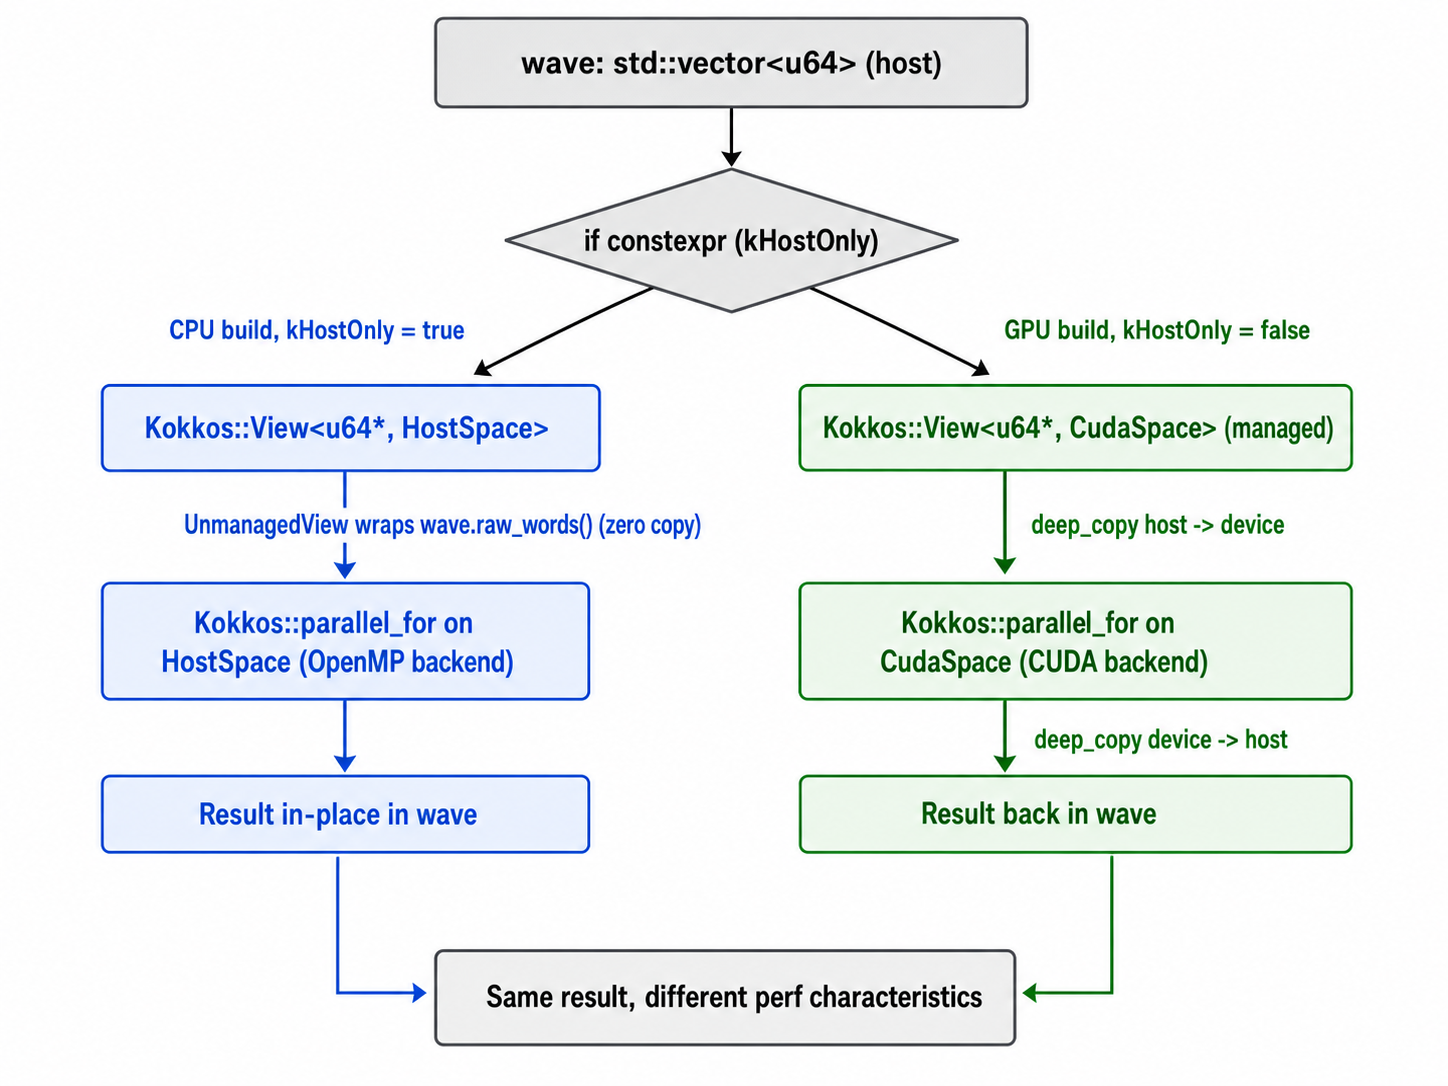
\includegraphics[width=\textwidth]{results/figures/schemas/kokkos_architecture.png}
\end{column}
\begin{column}{0.42\textwidth}
\textbf{Un seul code source}
\begin{itemize}
\footnotesize
    \item OpenMP, CUDA, HIP, SYCL
    \item \texttt{View<u64*, MemSpace>} pour la wave
    \item Functor \texttt{PropagateOp} : \texttt{KOKKOS\_INLINE\_FUNCTION}
\end{itemize}

\vspace{0.15cm}
\textbf{Branche \texttt{kHostOnly} compile-time}
\begin{itemize}
\footnotesize
    \item CPU : zero-copy (UnmanagedView wrap \texttt{wave.raw\_words()})
    \item GPU : \texttt{deep\_copy} host $\leftrightarrow$ device
    \item 0 overhead sur build CPU
\end{itemize}
\end{column}
\end{columns}
\end{frame}

% ============================================================
\begin{frame}[fragile]{Kokkos : contraintes GPU}
\begin{columns}[T]
\begin{column}{0.50\textwidth}
\textbf{Pas de heap dans le kernel}
\begin{itemize}
\footnotesize
    \item \texttt{new}, \texttt{vector::resize} interdits ou catastrophiques
    \item Stack arrays de taille connue compile-time
\end{itemize}

\begin{lstlisting}
constexpr size_t MAX_WORDS_PER_CELL = 8;

KOKKOS_INLINE_FUNCTION
void operator()(const int idx) const {
    const int c = frontier(idx);
    const int W = wave.words_per_cell;
    // Snapshot anti-race en stack
    uint64_t snap[MAX_WORDS_PER_CELL];
    for (int w = 0; w < W; ++w)
        snap[w] = wave.words(c*W + w);
    // ...
}
\end{lstlisting}
\end{column}
\begin{column}{0.46\textwidth}
\textbf{Optims OMP propagées}
\begin{itemize}
\footnotesize
    \item Snapshot anti-race : stack array
    \item Mask all-ones skip
    \item Relaxed-load skip avant \texttt{atomic\_fetch\_and}
    \item CAS dedup : \texttt{atomic\_compare\_exchange}
\end{itemize}

\vspace{0.15cm}
\textbf{\texttt{push\_finalize\_hook}}
\begin{itemize}
\footnotesize
    \item Évite View deallocated after \texttt{finalize}
    \item Caches \texttt{thread\_local} libérés \emph{pendant} le finalize
\end{itemize}
\end{column}
\end{columns}
\end{frame}

% ============================================================
\section{Extensions et démo UE5}

\begin{frame}{Extensions opt-in}
\begin{columns}[T]
\begin{column}{0.32\textwidth}
\begin{block}{Parallel attempts}
\texttt{--parallel-attempts K}
\begin{itemize}
\footnotesize
    \item K attempts WFC indépendants en parallèle
    \item Succès d'index minimum gagne (déterministe)
    \item \textbf{2.14$\times$} sur terrain N=3
\end{itemize}
\end{block}
\end{column}
\begin{column}{0.32\textwidth}
\begin{block}{Symétries D4}
\texttt{--symmetries S}
\begin{itemize}
\footnotesize
    \item $S \in \{1,2,4,8\}$
    \item Rotations + réflexions
    \item $L'$ peut atteindre $8 \times L$
    \item Hot path inchangé à $S=1$
\end{itemize}
\end{block}
\end{column}
\begin{column}{0.32\textwidth}
\begin{block}{Backtracking}
\texttt{--backtrack}
\begin{itemize}
\footnotesize
    \item Snapshot delta-encodé ($\sim 80\times$ moins de mémoire)
    \item Résout des instances où retry échoue
    \item Composable avec parallel-attempts
\end{itemize}
\end{block}
\end{column}
\end{columns}

\vspace{0.4cm}

\begin{itemize}
    \item Toutes \textbf{strictement opt-in} : zéro impact mesurable sur le chemin par défaut.
    \item Vérifiées par \texttt{test\_parallel\_attempts}, \texttt{test\_symmetries}, \texttt{test\_backtrack}.
\end{itemize}
\end{frame}

% ============================================================
\begin{frame}{Démo Unreal Engine 5}
\begin{columns}[T]
\begin{column}{0.55\textwidth}
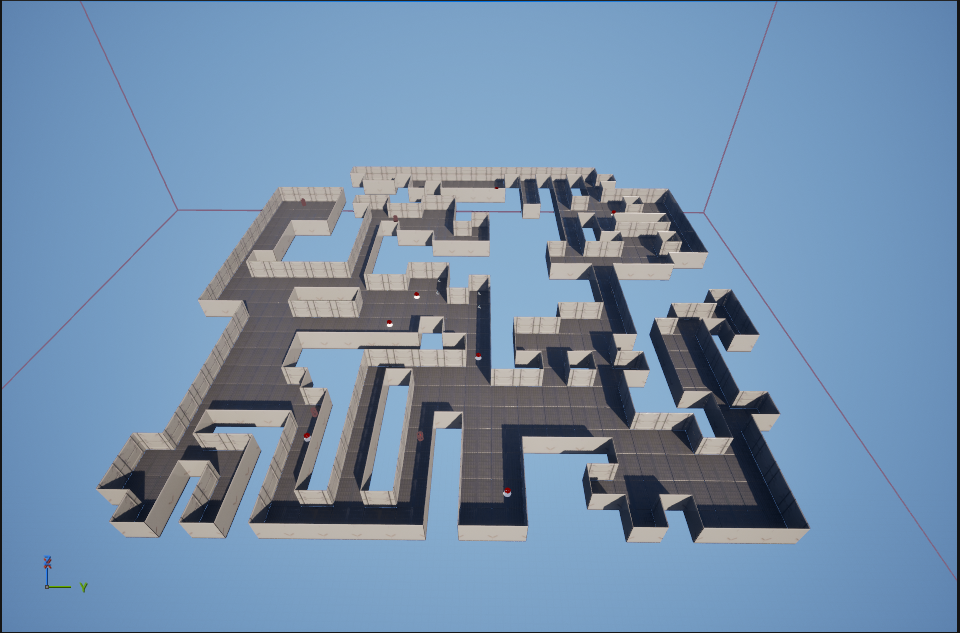
\includegraphics[width=\textwidth]{results/figures/ue5/ue5_dungeon_03.png}
\end{column}
\begin{column}{0.42\textwidth}
\textbf{Pipeline \texttt{wfc\_dungeon} $\to$ UE 5.7}
\begin{enumerate}
\footnotesize
    \item CLI émet JSON : grid + tile\_alphabet + cells + neighbors
    \item Connectivité walkable validée par flood-fill BFS
    \item Plugin parse, spawn \texttt{StaticMeshComponent} avec yaw cardinal
    \item Mesh variants par tile id
\end{enumerate}

\vspace{0.2cm}
\textbf{Gameplay scaffold}
\begin{itemize}
\footnotesize
    \item \texttt{PlayerStartClass}, \texttt{NPCSpawnerClass}, \texttt{PickupClass}
    \item Allocation non-collisionnelle
    \item \texttt{NavMeshBoundsVolume} auto-calculé
    \item Bouton \emph{Generate Random} (CallInEditor)
\end{itemize}
\end{column}
\end{columns}
\end{frame}

% ============================================================
\section{Résultats}

\begin{frame}{Protocole expérimental}
\begin{columns}[T]
\begin{column}{0.50\textwidth}
\begin{block}{Plate-forme principale -- Romeo}
\begin{itemize}
\footnotesize
    \item AMD EPYC 9654 (192c, 8 NUMA)
    \item \texttt{OMP\_PROC\_BIND=close}
    \item \texttt{OMP\_PLACES=cores}
\end{itemize}
\end{block}

\begin{block}{Plate-forme GPU -- Romeo armgpu}
\begin{itemize}
\footnotesize
    \item NVIDIA GH200 (132 SM, 16\,896 cores CUDA)
    \item ARM Grace (72c)
\end{itemize}
\end{block}
\end{column}
\begin{column}{0.46\textwidth}
\begin{block}{Variation systématique}
\begin{itemize}
\footnotesize
    \item Taille : 32 à 256 (timeout 4h à 512)
    \item Sample : binary\_L11, terrain\_L33, smooth\_N3
    \item Threads : 1, 2, 4, 8, 16, 32, 64, 192
    \item Backend : serial, omp, kokkos
\end{itemize}
\end{block}

\vspace{0.2cm}
\textbf{220+ runs SLURM benchmarkés}\\
{\footnotesize Médiane sur 3 répétitions ; A/B critiques sur 11 runs alternés.}
\end{column}
\end{columns}
\end{frame}

% ============================================================
\begin{frame}{Speedup binary\_L11 sur Romeo}
\begin{columns}[T]
\begin{column}{0.55\textwidth}

\includegraphics[width=\textwidth]{results/figures/scaling/speedup_binary_L11.png}
\end{column}
\begin{column}{0.42\textwidth}
\begin{block}{Strong scaling Romeo}
\centering
\footnotesize
\begin{tabular}{lrrr}
\toprule
\textbf{Taille} & \textbf{8t} & \textbf{16t} & \textbf{Peak} \\
\midrule
32$\times$32   & 0.91$\times$ & 0.33$\times$ & 1.16$\times$ (4t) \\
64$\times$64   & 2.64$\times$ & 0.65$\times$ & 2.64$\times$ \\
128$\times$128 & \textbf{5.27$\times$} & 2.60$\times$ & 5.27$\times$ \\
256$\times$256 & 6.73$\times$ & \textbf{8.23$\times$} & \textbf{8.23$\times$} \\
\bottomrule
\end{tabular}
\end{block}

\vspace{0.2cm}
\textbf{Peak 8.23$\times$ à 16 threads sur 256$\times$256} (51\% d'efficacité). Régression au-delà : fork/join + contention atomique cross-NUMA.
\end{column}
\end{columns}
\end{frame}

% ============================================================
\begin{frame}{Heatmap et fit Amdahl}
\begin{columns}[T]
\begin{column}{0.48\textwidth}

\includegraphics[width=\textwidth]{results/figures/scaling/heatmap_binary_L11.png}\\[2pt]
{\scriptsize Sweet spot diagonal : taille optimale suit le thread count.}
\end{column}
\begin{column}{0.48\textwidth}
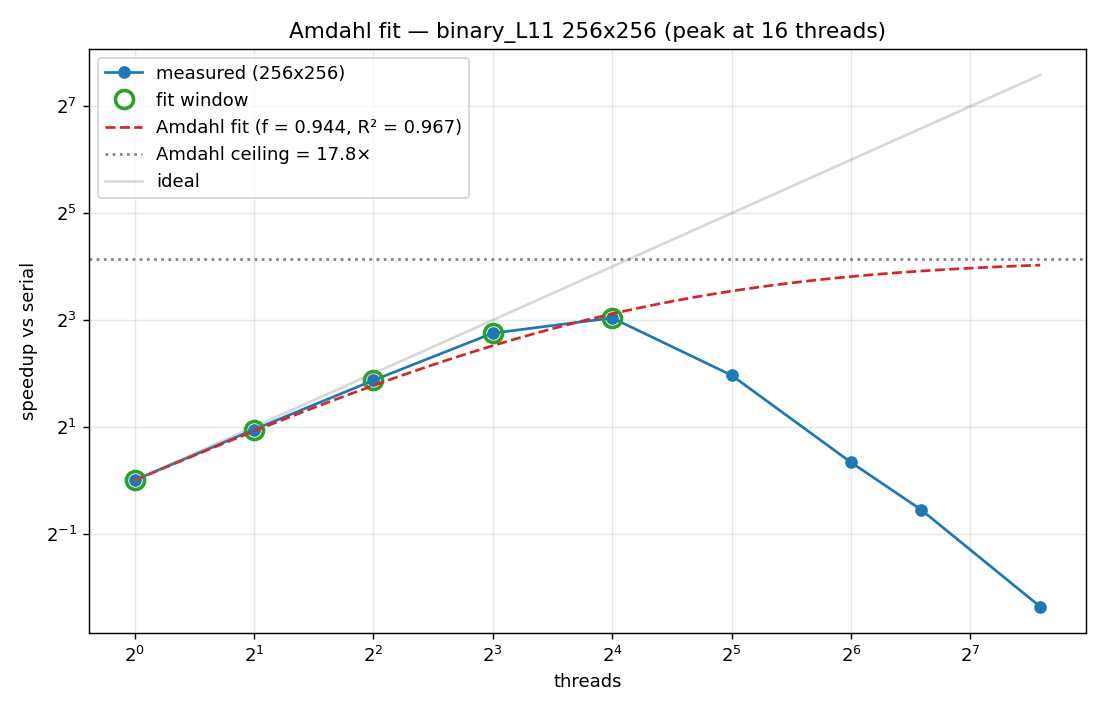
\includegraphics[width=\textwidth]{results/figures/amdahl/amdahl_binary_L11_256.png}\\[2pt]
{\scriptsize Fit Amdahl 256 : $f = 0.944$, ceiling $17.8\times$, peak $8.23\times$ (46\% du ceiling).}
\end{column}
\end{columns}

\vspace{0.2cm}
\textbf{Coûts \emph{supra}-Amdahl} expliquent l'écart au ceiling : fork/join, contention atomique cross-NUMA, frontières BFS courtes. Ces coûts ne sont pas modélisés par Amdahl.
\end{frame}

% ============================================================
\begin{frame}{Comparaison serial / OMP / Kokkos}
\begin{columns}[T]
\begin{column}{0.48\textwidth}
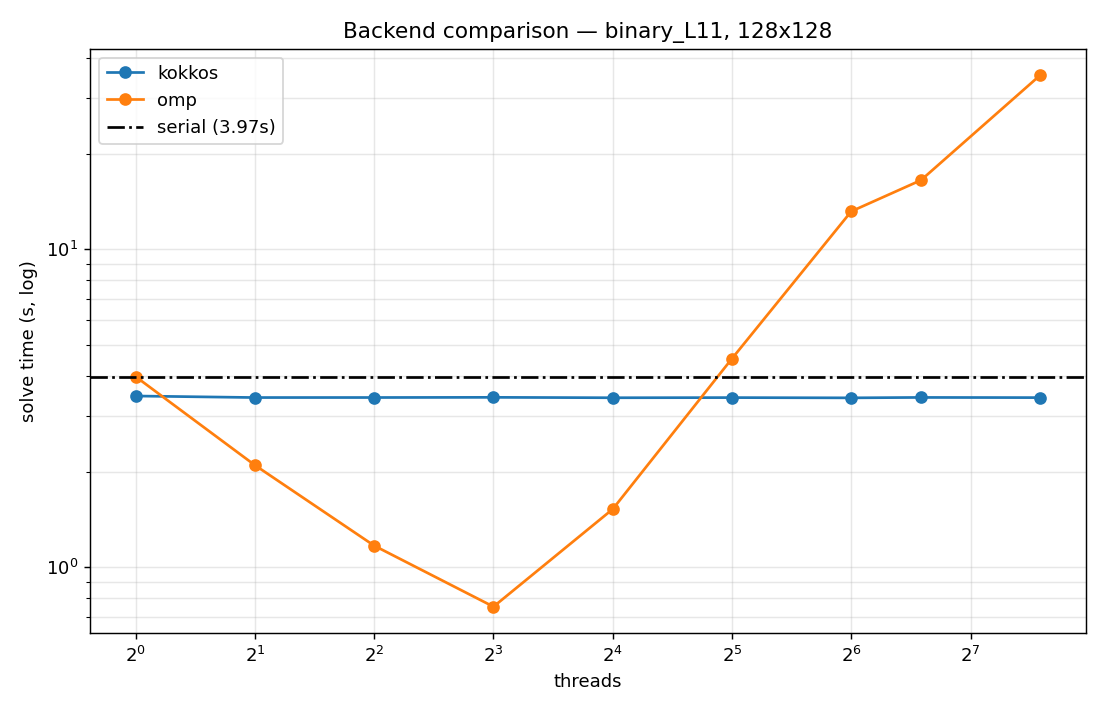
\includegraphics[width=\textwidth]{results/figures/scaling/backends_binary_L11_128.png}\\[2pt]
{\scriptsize binary\_L11 128$\times$128, échelle log.}
\end{column}
\begin{column}{0.48\textwidth}
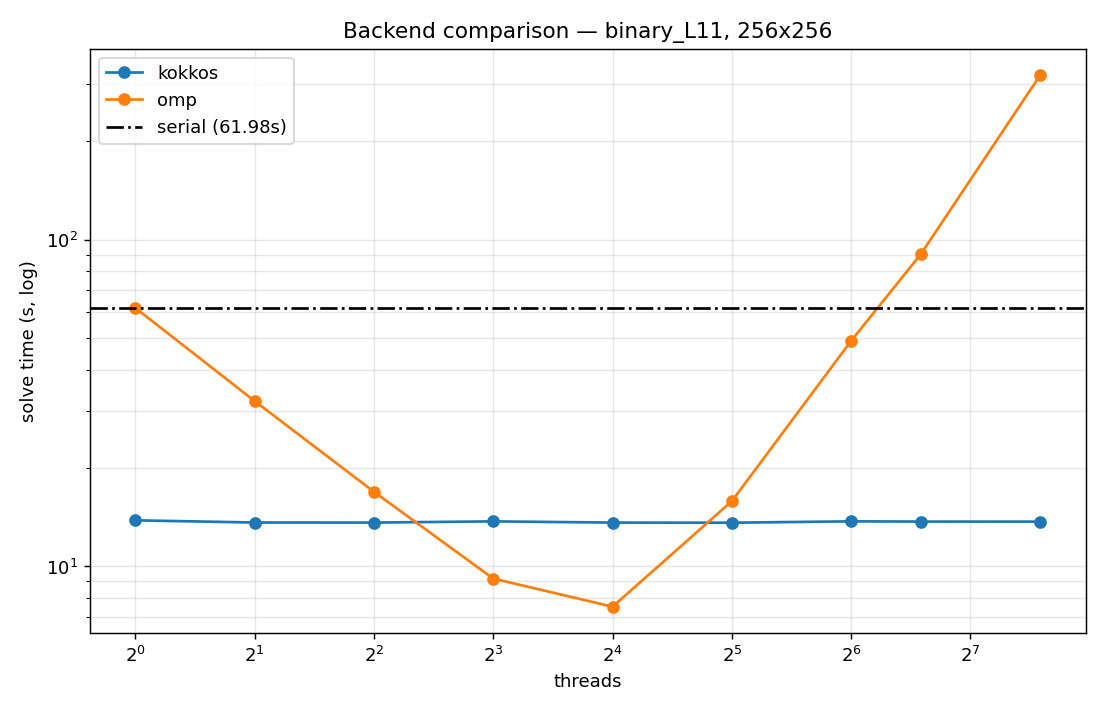
\includegraphics[width=\textwidth]{results/figures/scaling/backends_binary_L11_256.png}\\[2pt]
{\scriptsize binary\_L11 256$\times$256, échelle log.}
\end{column}
\end{columns}

\vspace{0.2cm}
\begin{itemize}
    \item OMP $>$ Kokkos sur ce workload : overhead Views + dispatch.
    \item Kokkos converge vers OMP sur grandes tailles (le travail amortit l'overhead).
    \item Kokkos GPU 8$\times$ plus lent que OMP CPU sur 128 : H$\leftrightarrow$D copies par \texttt{propagate} dominent.
\end{itemize}
\end{frame}

% ============================================================
\begin{frame}{Galerie de sorties WFC}
\begin{columns}[T]
\begin{column}{0.32\textwidth}
\centering

\includegraphics[height=2.6cm]{results/figures/results/gallery/rooms_seed42.png}\\[1pt]
{\scriptsize rooms ($N=3$, binaire)}
\end{column}
\begin{column}{0.32\textwidth}
\centering
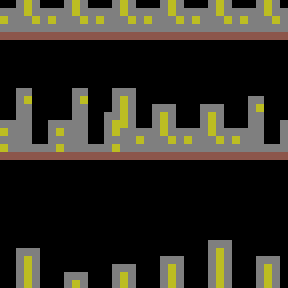
\includegraphics[height=2.6cm]{results/figures/results/gallery/skyline_seed42.png}\\[1pt]
{\scriptsize skyline ($N=3$, 4 valeurs)}
\end{column}
\begin{column}{0.32\textwidth}
\centering
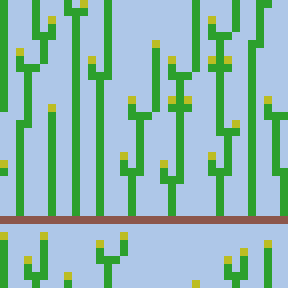
\includegraphics[height=2.6cm]{results/figures/results/gallery/plant_seed42.png}\\[1pt]
{\scriptsize plant ($N=3$, 4 valeurs)}
\end{column}
\end{columns}

\vspace{0.2cm}

\begin{columns}[T]
\begin{column}{0.32\textwidth}
\centering

\includegraphics[height=2.4cm]{results/figures/results/binary_5x5_64x64_N2_seed42.png}\\[1pt]
{\scriptsize binary\_5x5 (sujet, $N=2$)}
\end{column}
\begin{column}{0.32\textwidth}
\centering
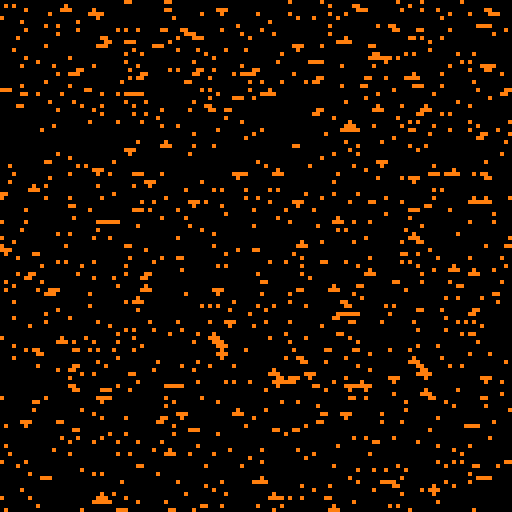
\includegraphics[height=2.4cm]{results/figures/results/multivalue_terrain_128x128_N2_seed11.png}\\[1pt]
{\scriptsize terrain ($N=2$, 33 tuiles)}
\end{column}
\begin{column}{0.32\textwidth}
\centering

\includegraphics[height=2.4cm]{results/figures/results/multivalue_smooth_64x64_N3_seed19.png}\\[1pt]
{\scriptsize smooth ($N=3$, gradients)}
\end{column}
\end{columns}

\vspace{0.1cm}
{\footnotesize Tous obtenus avec \texttt{wfc\_serial} (bit-identique en OMP/Kokkos).}
\end{frame}

% ============================================================
\section{Conclusion}

\begin{frame}{Conclusion}
\begin{columns}[T]
\begin{column}{0.55\textwidth}
\textbf{Speedup peak : 8.23$\times$} (16 threads, 256$\times$256, Romeo)

\vspace{0.3cm}
\textbf{Optims gardées}
\begin{enumerate}
\footnotesize
    \item Une seule région \texttt{parallel} pour propagation (essentiel)
    \item Frontier-threshold : $+25\%$ à 64t, $+29\%$ à 192t
    \item Atomic relaxed-load skip : $-50\%$ trafic atomique
    \item Per-thread frontier \texttt{alignas(64)} (anti-faux-partage)
    \item LTO : $+3.4\%$ médiane sur 11 runs
\end{enumerate}

\vspace{0.3cm}
\textbf{Validation}
\begin{itemize}
\footnotesize
    \item 24\,980 invariants vérifiés, 99\% line coverage
    \item Déterminisme bit-à-bit serial = OMP = Kokkos
    \item 220+ runs Romeo benchmarkés
\end{itemize}
\end{column}
\begin{column}{0.42\textwidth}
\textbf{Limites}
\begin{itemize}
\footnotesize
    \item Régression au-delà de 32t (contention NUMA)
    \item smooth\_N3 plafonne ($f = 0.74$)
    \item GPU GH200 plus lent que CPU sur ce workload
\end{itemize}

\vspace{0.3cm}
\begin{block}{Pistes d'amélioration}
\begin{itemize}
\footnotesize
    \item Entropie incrémentale (PQ) : facteur $\sim 1000$ sur la phase qui domine
    \item NUMA partitioning : peak attendu $12$-$14\times$ à 64t
    \item Batch GPU : K solveurs $\to$ data-parallelism massif
\end{itemize}
\end{block}
\end{column}
\end{columns}
\end{frame}

% ============================================================
\begingroup
\setbeamertemplate{frametitle}{}
\usebackgroundtemplate{%
  \begin{tikzpicture}[remember picture,overlay]
    \node[opacity=0.20, anchor=center] at (current page.center) {%
      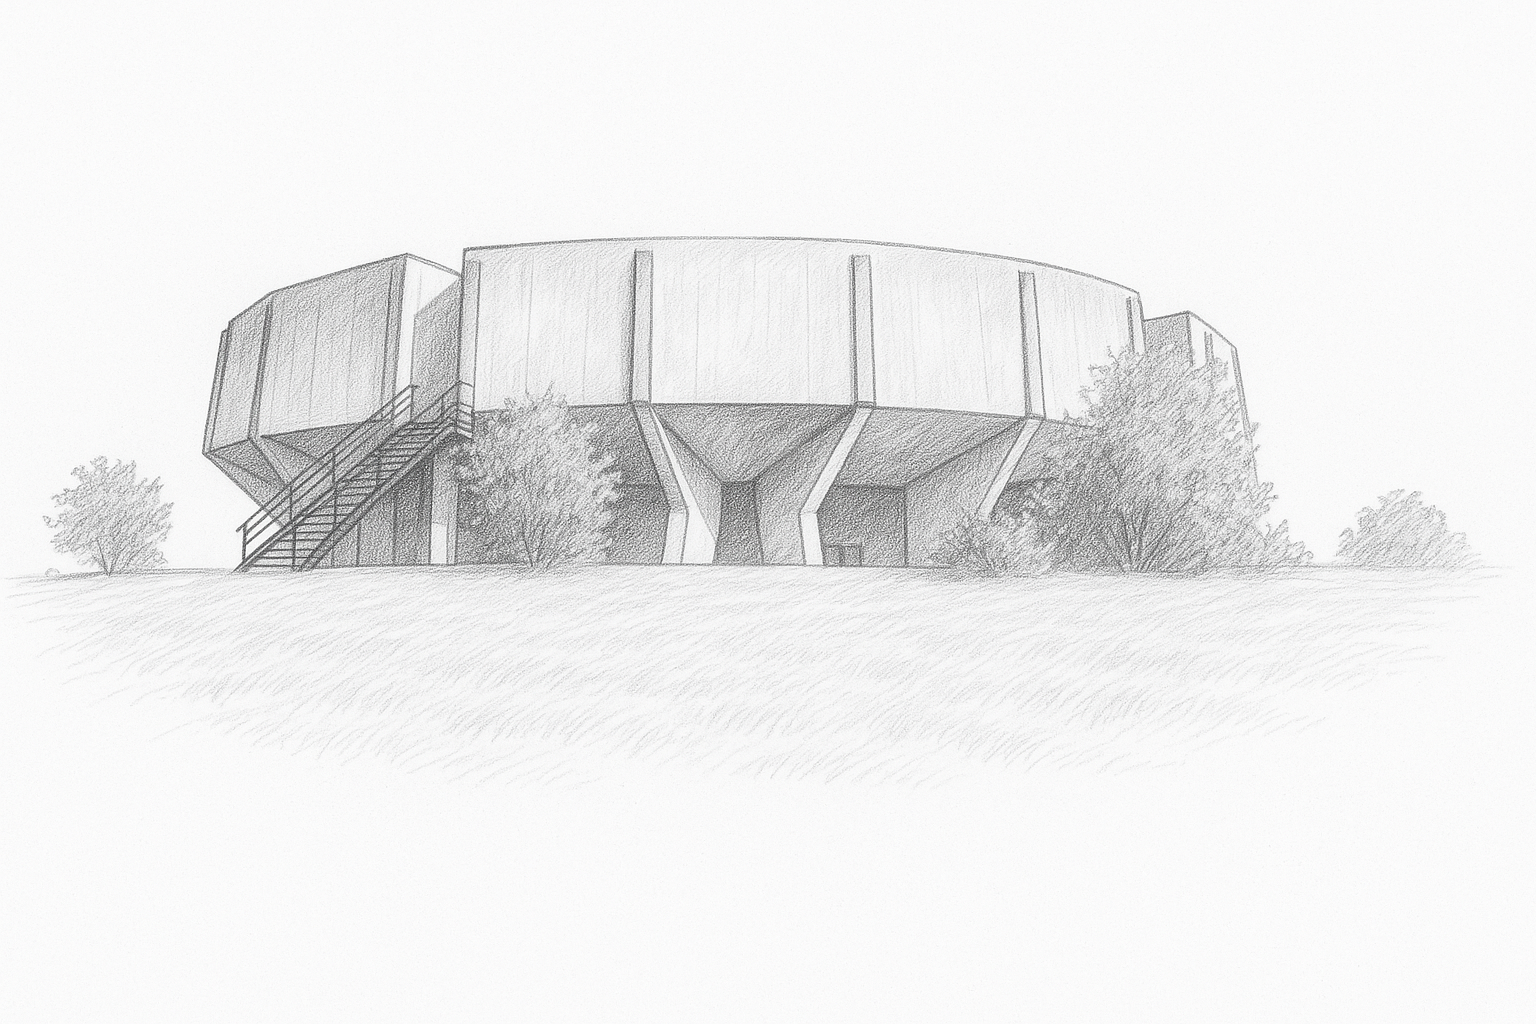
\includegraphics[width=\paperwidth,keepaspectratio]{assets/back.png}%
    };
  \end{tikzpicture}%
}
\begin{frame}{}
\vfill
\begin{center}
{\Large\color{burgundy}\bfseries Merci.}\\[0.5cm]
{\itshape Wave Function Collapse -- CHPS0801}\\[0.2cm]
{\small Romain Despoullains \& Nicolas Marano}
\end{center}
\vfill
\begin{center}

\includegraphics[height=1.5cm]{assets/logo-urca.png}
\end{center}
\vfill
\end{frame}
\endgroup

\end{document}
